\documentclass{beamer}
\usepackage{ dsfont }
\usepackage[utf8]{inputenc}
\usepackage{animate}
\usepackage{minted}
\usepackage{movie15}
\usepackage{breqn}
\usepackage{tcolorbox, amsmath}
\usepackage{subcaption}
\usepackage[english]{babel}
\setbeamersize{text margin left=10pt, text margin right=10pt} %new code
\usepackage{graphicx}
\usepackage{float}
\usepackage{subcaption}
\usefonttheme{professionalfonts} % using non standard fonts for beamer
\setbeamerfont{frametitle}{series=\bfseries}
\usepackage{animate}
\usepackage{movie15}
\usepackage{breqn, bm}
\usepackage{amsmath}

\definecolor{notgreen}{RGB}{255,127,0}
\definecolor{green}{RGB}{49,150,3}
\setbeamerfont{headline}{size=\small}


%----------------------------------------------------------------------------------------
%	 Package
%----------------------------------------------------------------------------------------
\usepackage{color}
\usepackage{url}
\beamertemplatenavigationsymbolsempty
\definecolor{cadmiumred}{rgb}{0.8, 0.8, 0.8}

%----------------------------------------------------------------------------------------
%	 Presentation settings
%----------------------------------------------------------------------------------------

\usetheme{default}
\usecolortheme{default}

\setbeamertemplate{itemize items}[triangle] 
\setbeamertemplate{enumerate items}[default]
 
\title[Variational Drop Out]{
	MIPT Data Visualization Course\\ 
	\vspace{1cm}
	\textbf{\textcolor{black}{Deep Learning for Data with Sequence Structure}}}

\author{Ashuha Arseniy$^{1, 2}$}
\institute[Bayesgroup, MIPT]{
	Bayesian Research Group$^1$, MIPT$^2$\\
	
	\medskip
	
\includegraphics[scale=0.5]{./img/logo} 
\includegraphics[scale=0.12]{./img/mipt}
	
	\href{ars-ashuha.ru/slides}{ars-ashuha.ru/slides}}

\date{\today}

\newcommand{\Expect}{\mathsf{E}}
\newcommand{\MExpect}{\mathsf{M}}
\newcommand{\cov}{\mathsf{cov}}
\setbeamertemplate{section in toc}[circle]

\addtobeamertemplate{navigation symbols}{}{%
	\usebeamerfont{footline}%
	\usebeamercolor[fg]{footline}%
	\hspace{1em}%
	\insertframenumber/\inserttotalframenumber
}


\begin{document}

\begin{frame}
	\titlepage 
\end{frame}

\begin{frame}{Independent and Identically-Distributed}
	\begin{itemize}
		 \item Image classification
		\begin{center}
			 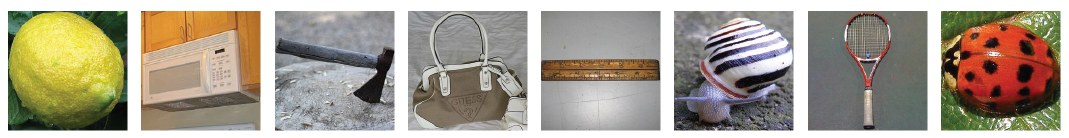
\includegraphics[scale=2]{./img/ims}
		\end{center}
		\item Flicker user's image classification 
			
	\end{itemize}
	\begin{figure}
		\begin{subfigure}{.4\textwidth}
			\centering 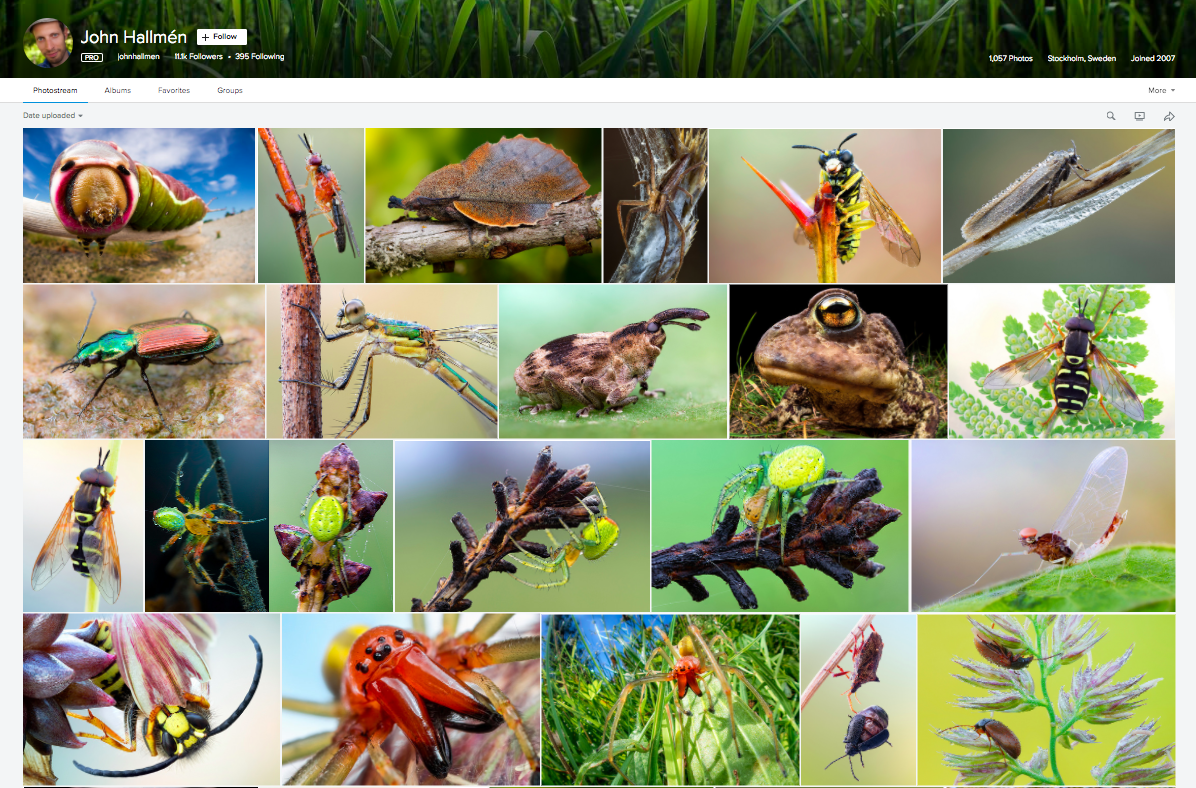
\includegraphics[scale=0.1]{img/fl1} 
		\end{subfigure}
		 
		\begin{subfigure}{.49\textwidth}
			\centering 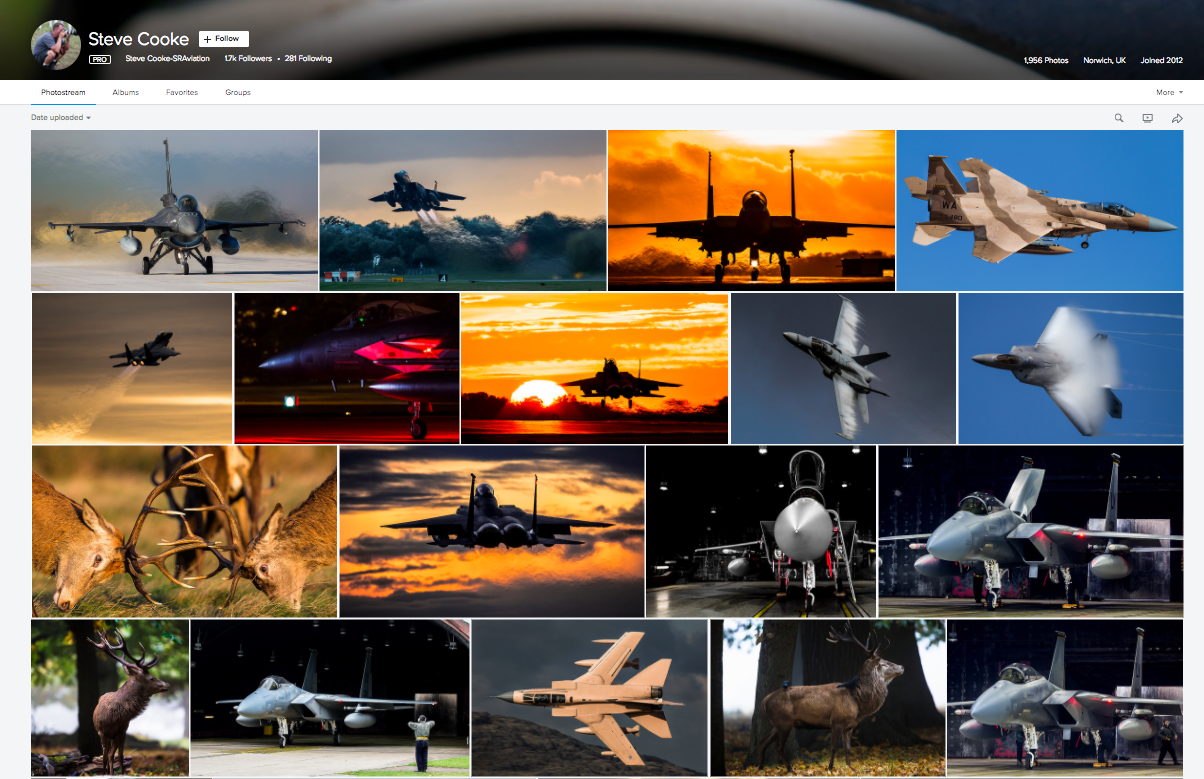
\includegraphics[scale=0.1]{img/fl4} 
		\end{subfigure}
	\end{figure}
\end{frame}

\begin{frame}{Flicker user's image classification }
	
	\begin{itemize}
			 \item Now we need to classify objects jointly, so we had sequence on input
			\begin{center}
				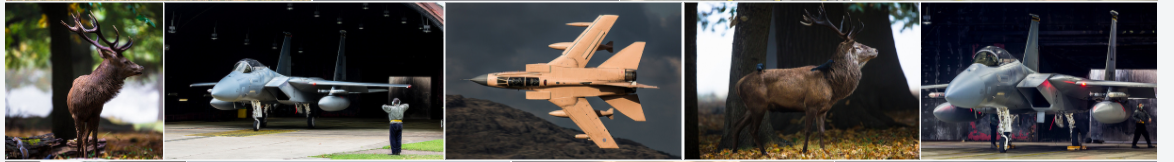
\includegraphics[scale=0.27]{./img/fl5}
			\end{center}
			
			 \item and predict sequence
			\begin{center}
				\texttt{['deer', 'plane',  'plane', 'deer',  'plane']}
			\end{center}
			 \item What should we do? Do you have any ideas? 
			 \item Lets apply CNN for each image to get descriptor.
			 \begin{center}
				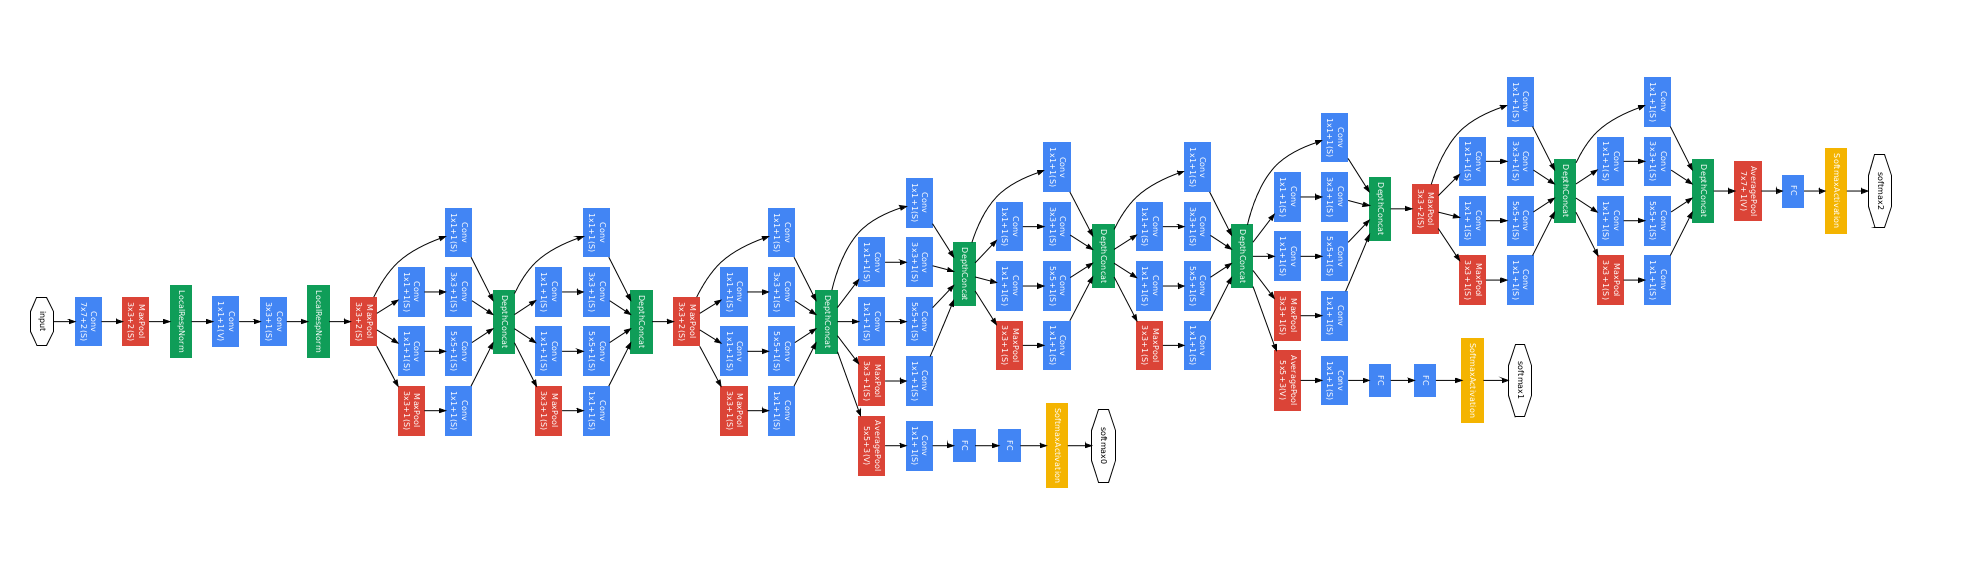
\includegraphics[scale=0.27]{./img/gln}
			\end{center}
			 \item We've transform sequence of pictures so sequence of vectors
			 \item Ok data became much simply, what's next?
	\end{itemize}	
\end{frame}

\begin{frame}[fragile]{Recurrent Neural Net Concept}
	\begin{itemize}
		\item   Let's introduce memory cell 
		 
		\begin{center}
			\begin{minted}[fontsize=\small, frame=lines,
			framesep=2mm]{python}
memory = np.ones(num_class)
for pic_vec in ['pic1_vec', 'pic2_vec', 'pic3_vec']:
    pic_class = g(W.dot(pic_vec) * f(memory))
    memory[pic_class] += 1
			\end{minted}
		\end{center}
		\item   Hmm, we will try control memory automatic
		 
		\begin{center}
			\begin{minted}[fontsize=\small, frame=lines,
framesep=2mm]{python}
memory = np.ones(100)
for pic_vec in ['pic1_vec', 'pic2_vec', 'pic3_vec']:
    pic_class = g(Wout.dot([pic_vec, memory]))
    memory += Win.dot(pic_vec) + sigmoid(Wmem.dot(memory))
			\end{minted}
		\end{center}
		
		\item  Let's plot (memory update it's a little bit different but still it's same)
		 \begin{center}
			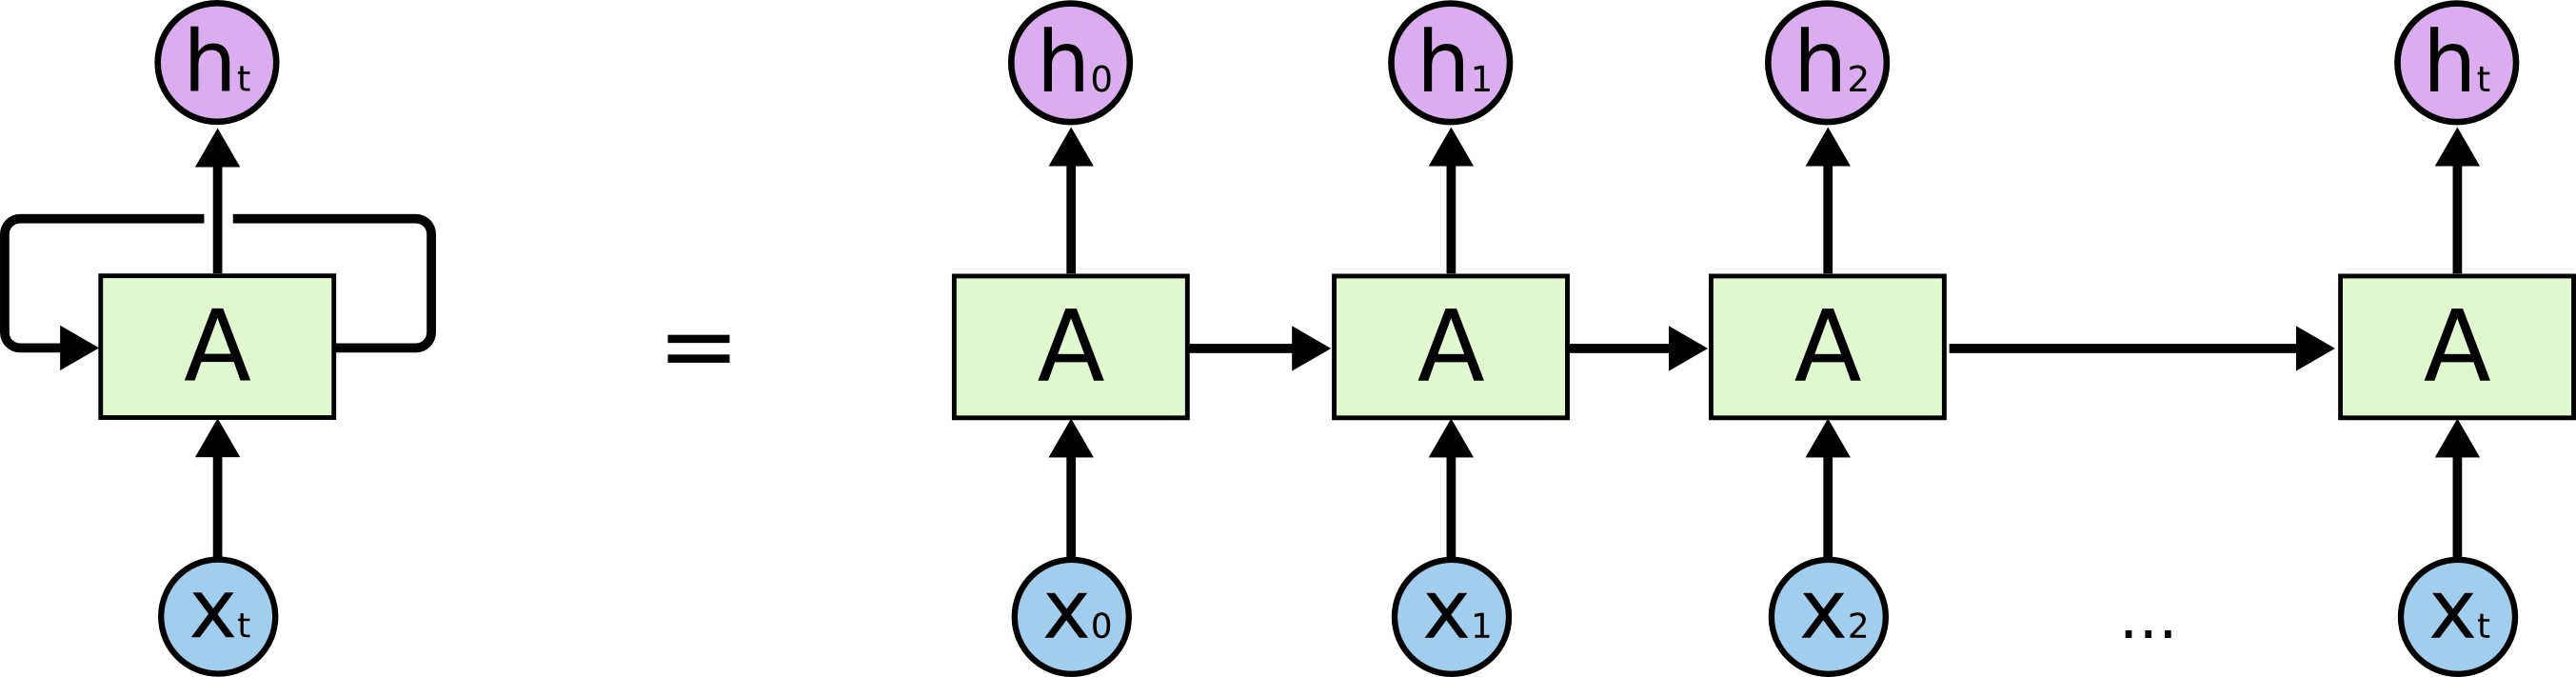
\includegraphics[scale=0.2]{./img/rnn_ur}
		\end{center}
	\end{itemize}
\end{frame}


\begin{frame}{RNN and Training}
	\begin{center}
		 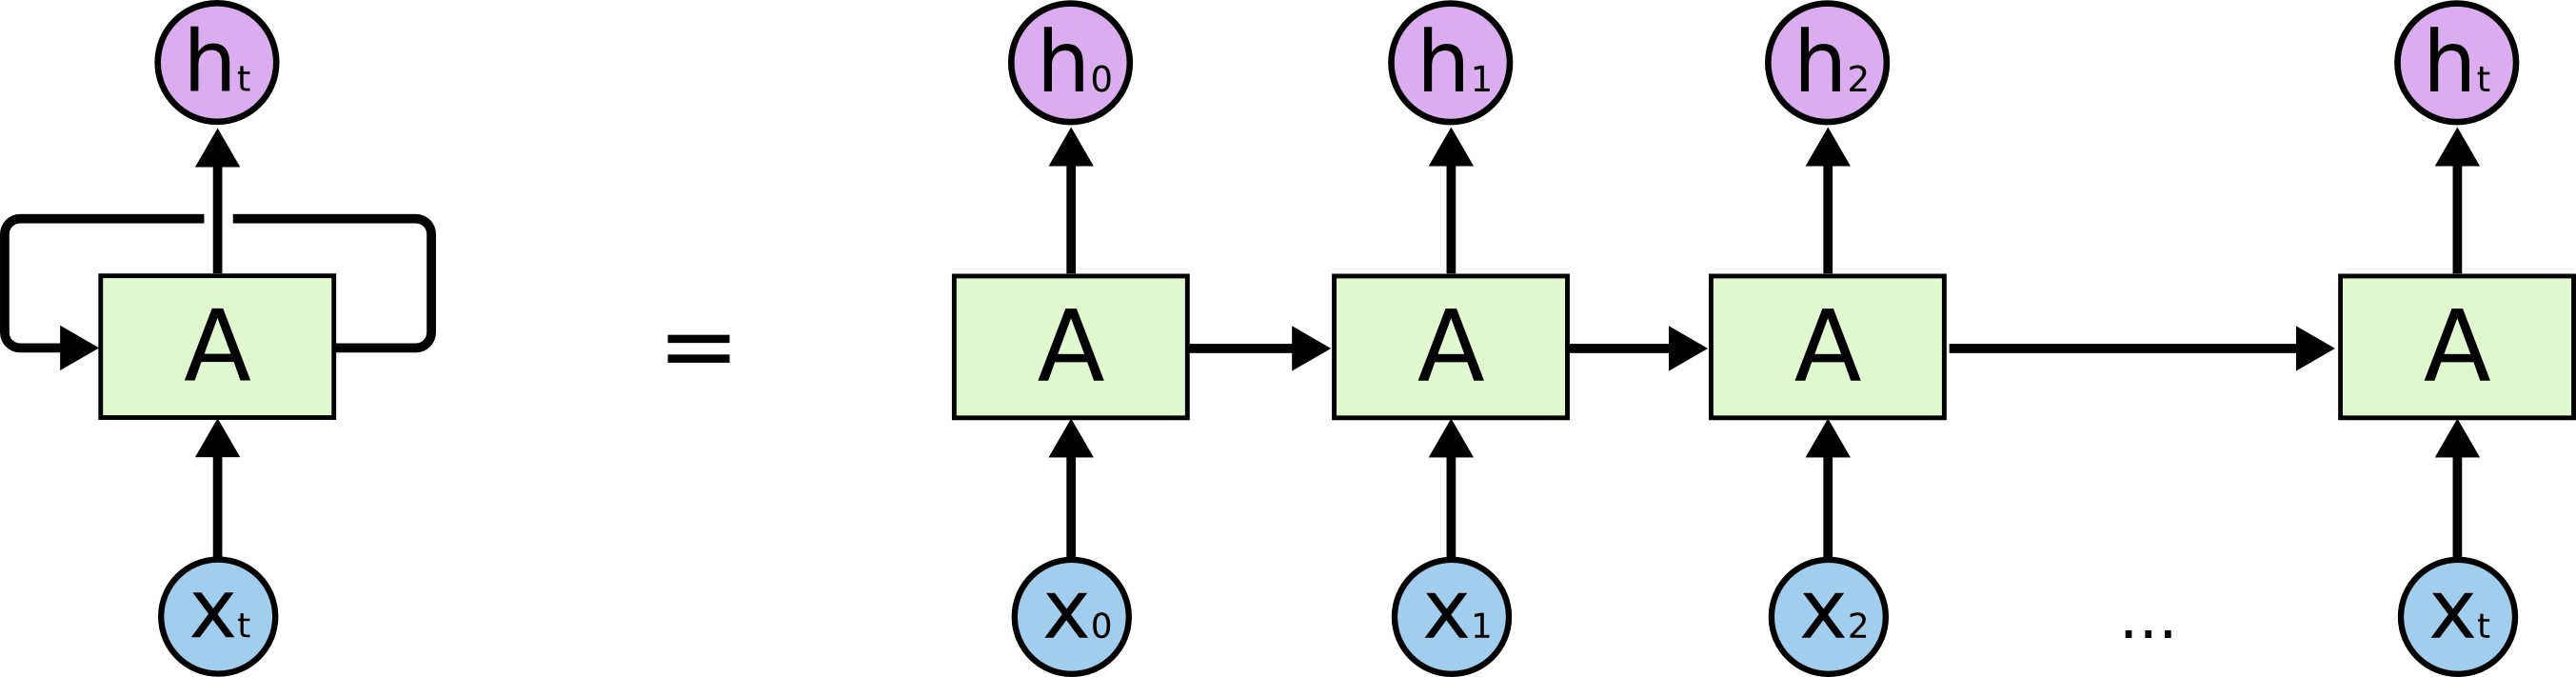
\includegraphics[scale=0.23]{./img/rnn_ur}
	\end{center}
	\begin{itemize}
		 \item So we can compute inputs-outputs using this equations
		 $$h_n = \textcolor{green}{W_x} x_n + \textcolor{red}{W_h}\sigma(h_{n-1})~~~\hat{y}_n = \sigma(\textcolor{notgreen}{W_y}  h_n) ~~ \theta = (W_x, W_h, W_y)$$
		\vspace{-0.6cm}
		 \item You get several inputs and outputs, how would you train RNNs?
		 \item Let's sum error for each output
		  $$L = \sum_t L_t(\hat{y}_t(\theta), y_t),~~~ \frac{\partial L }{\partial \theta} = \sum_{1 < t < T}  \frac{\partial L_T(\hat{y}_t(\theta), y_t) }{\partial \theta}$$ 
		 \item Next we should use ordinary optimization methods
	\end{itemize} 
\end{frame}

\begin{frame}{RNN and Training}
	\begin{center}
		 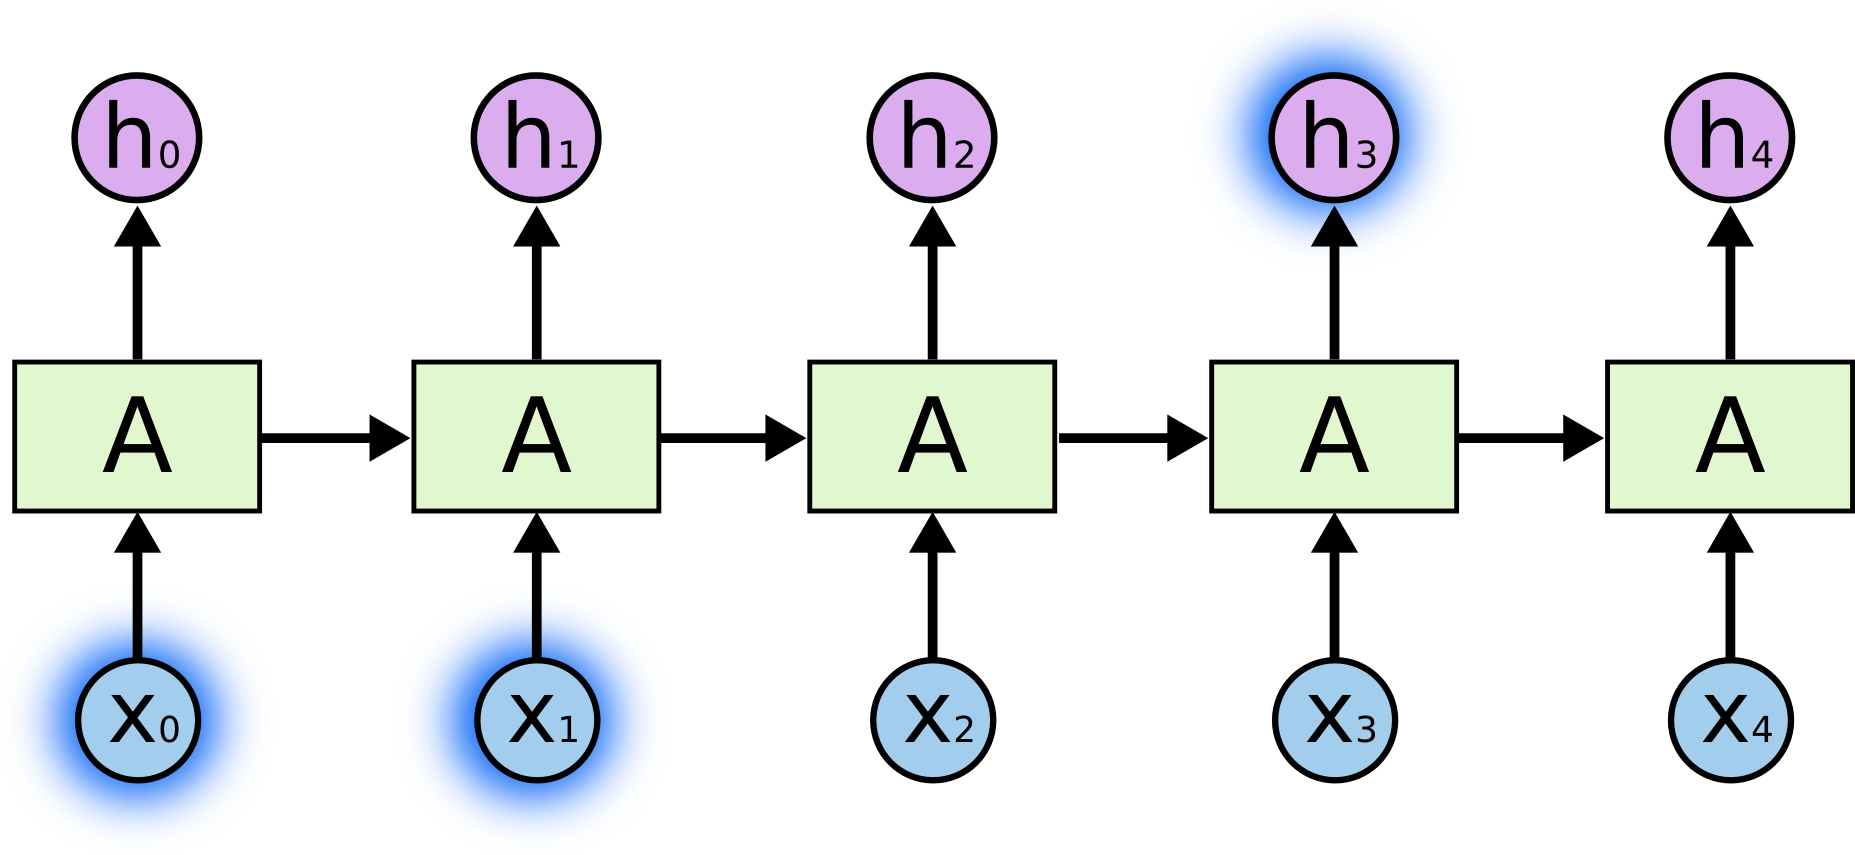
\includegraphics[scale=0.18]{./img/rnn_st}
		
		 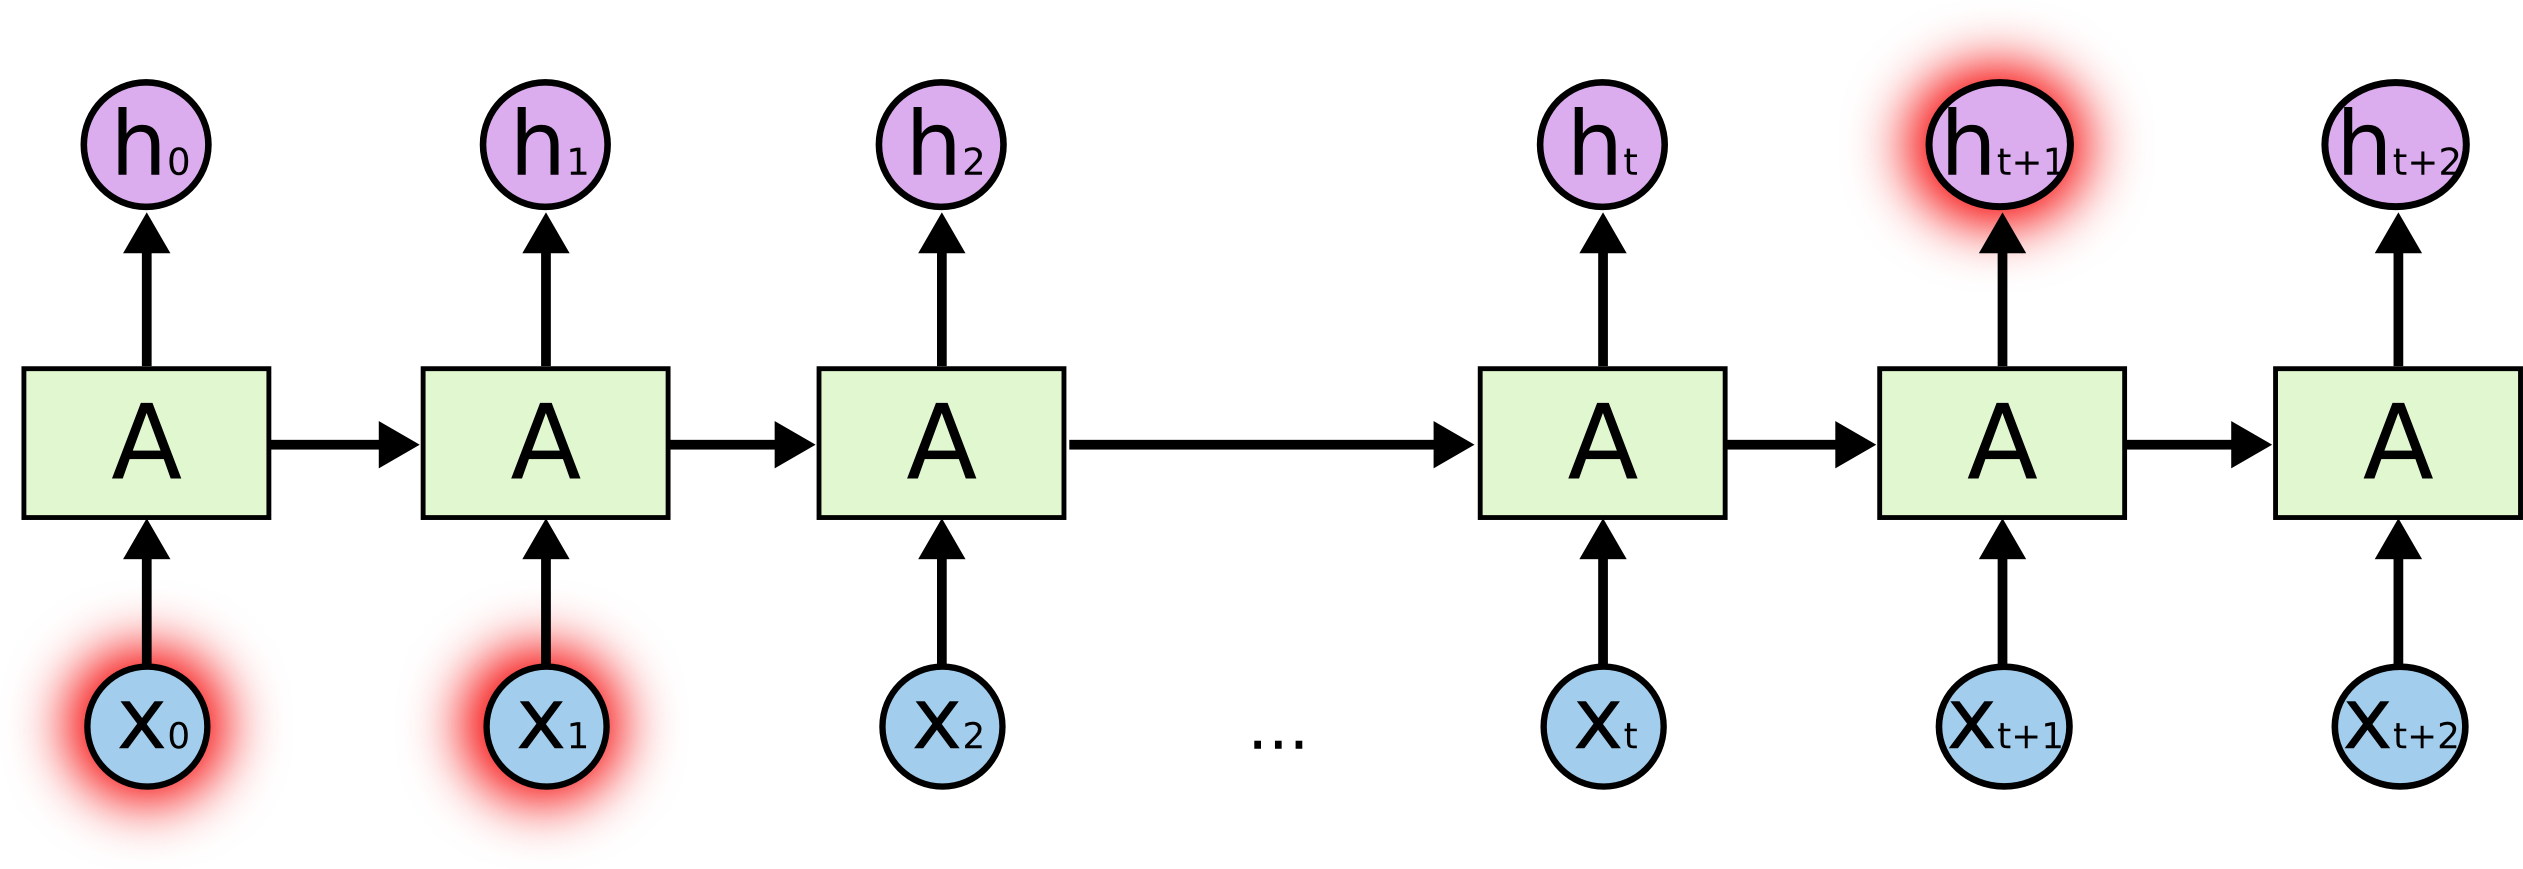
\includegraphics[scale=0.18]{./img/rnn_lt}
	\end{center}
	\begin{itemize}
		 \item Gradient is like this 
				  $$\frac{\partial E_t}{\partial \theta} = 
				\sum_{1 \leq k \leq  t}  \frac{\partial E_t}{\partial h_t} \frac{\partial h_t}{\partial h_k}
				\frac{\partial h_k}{\partial \theta} ~~~~\frac{\partial h_t}{\partial h_k} = \prod_{t\geq i \geq k} \frac{\partial h_i}{\partial h_{i-1}}$$		
		 \item Multiply on matrix with small norm means no long deps
		 \item Multiply on matrix with big norm means Gradient Boom
		
	 	\vspace{0.5cm}
		{\tiny Razvan Pascanu, Tomas Mikolov, Yoshua Bengio: On the difficulty of training recurrent neural networks}
	\end{itemize} 
\end{frame}

\begin{frame}{Dealing with gradients Boom}
	\begin{itemize}
		 \item What is the simplest solution?
		 \item Gradient clipping :)
			 \begin{center}
				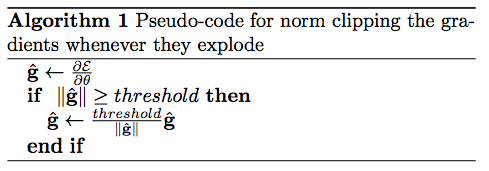
\includegraphics[scale=0.5]{./img/grad_clip}
			\end{center}
		 \item It really works while gradient variance is low
	\end{itemize}
	
		 \vspace{0.5cm}
		{\tiny Razvan Pascanu, Tomas Mikolov, Yoshua Bengio: On the difficulty of training recurrent neural networks}
\end{frame}

\begin{frame}{Dealing with long term dependences means LSTM}
	\begin{itemize}
		 \item We can't forget
		 \item We can't understand importance of input information
		 \item Let's add it 
	\end{itemize}
	\begin{center}
		 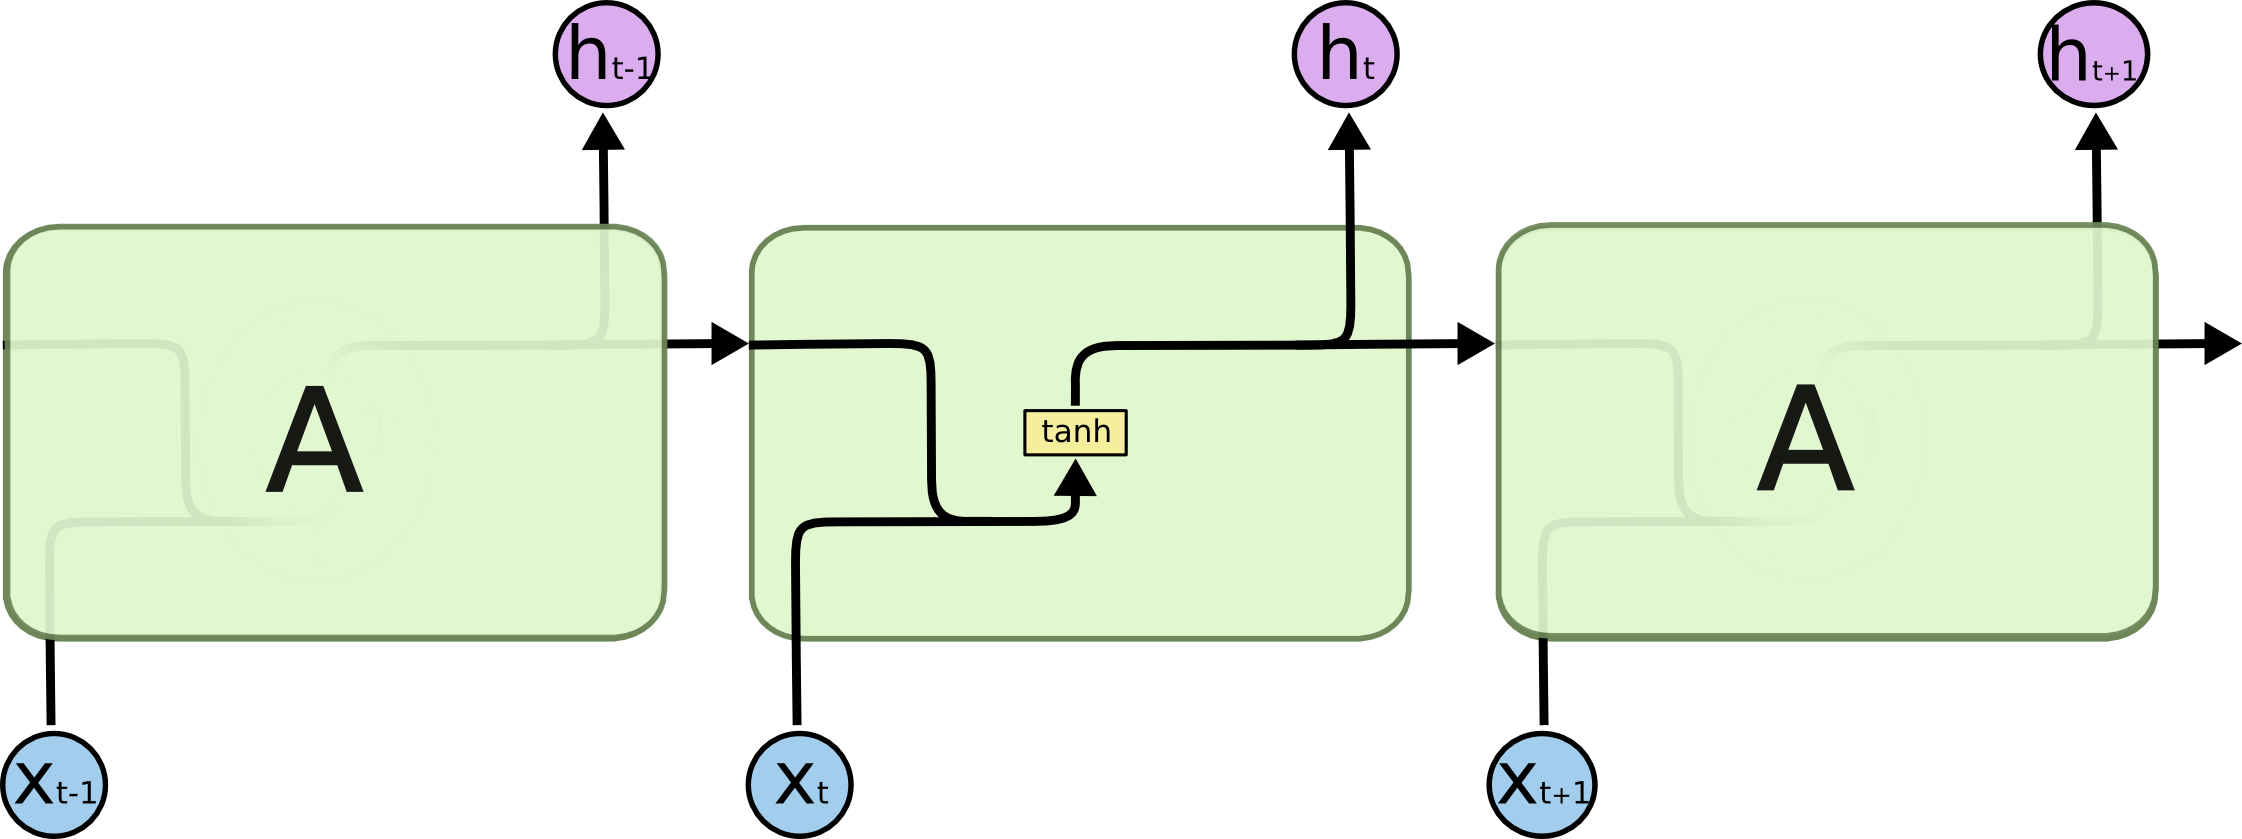
\includegraphics[scale=0.25]{./img/lstm_rnn}
		
		 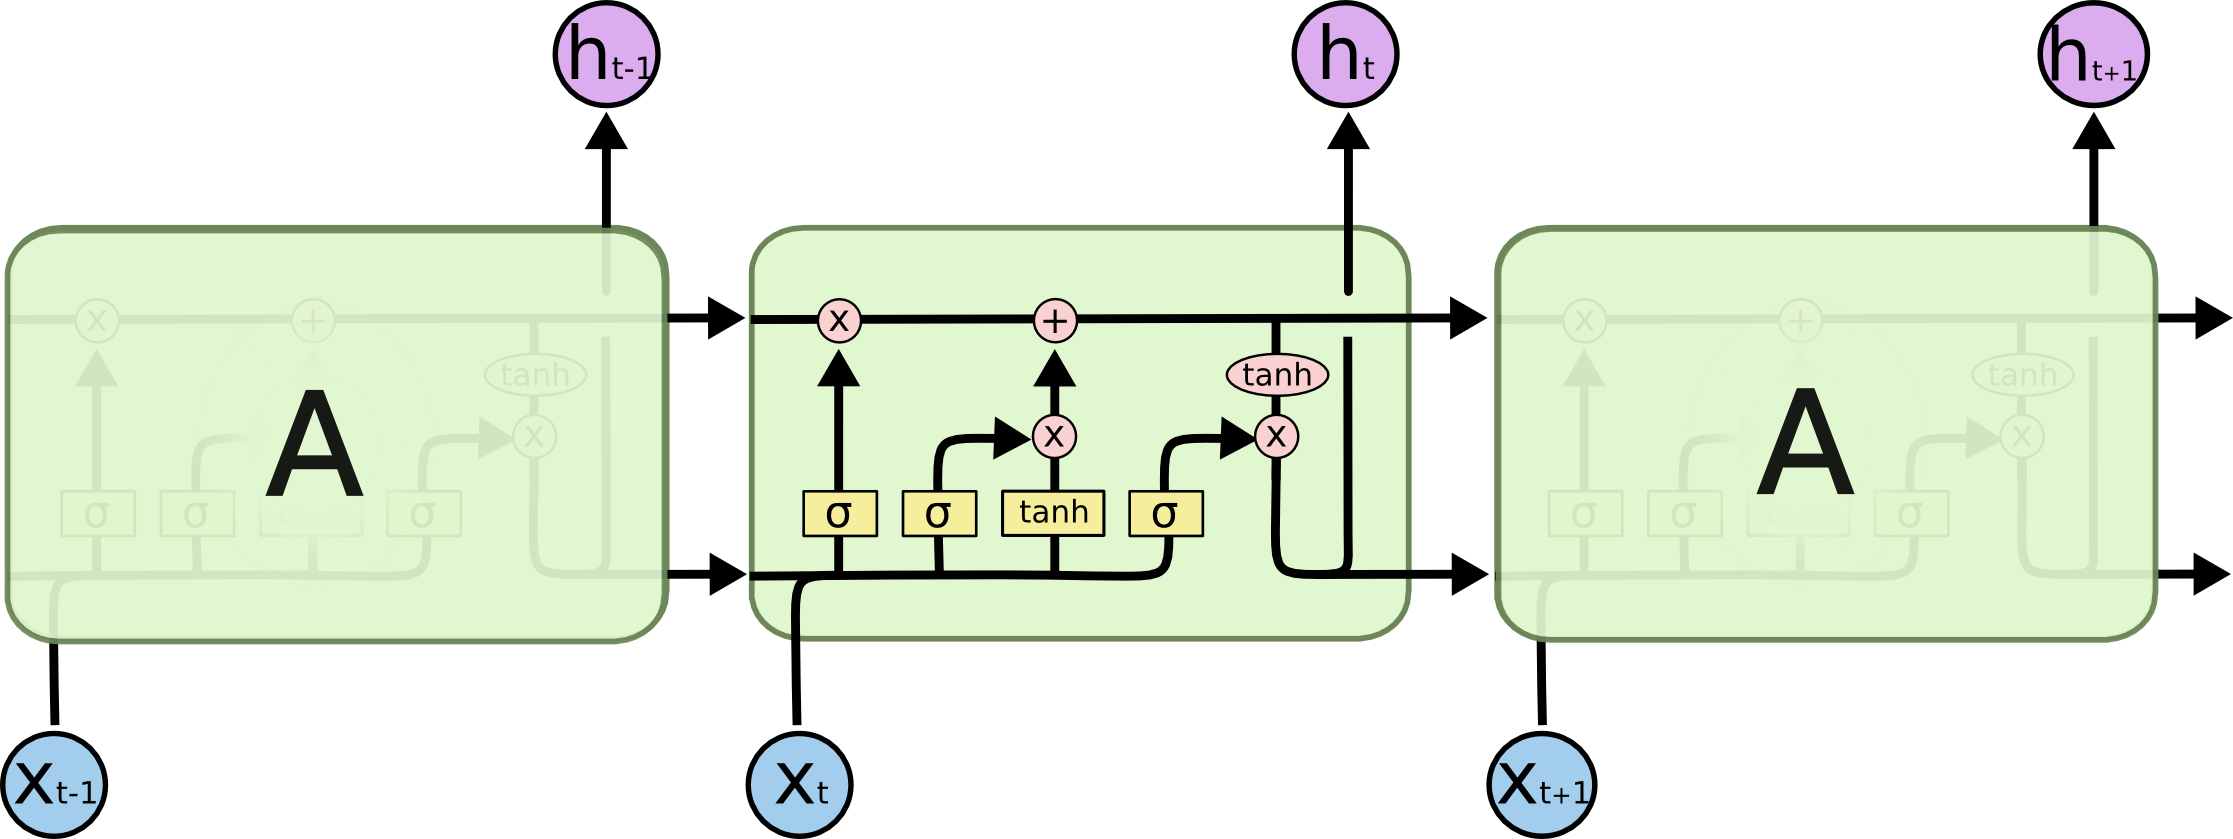
\includegraphics[scale=0.25]{./img/lstm_full}
		
		 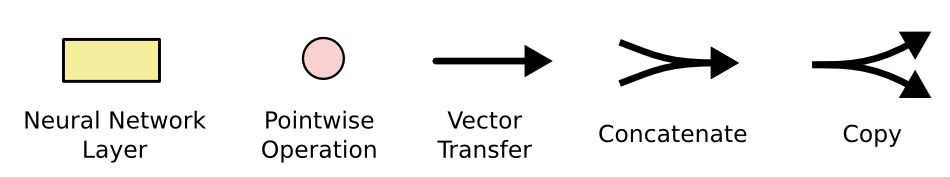
\includegraphics[scale=0.25]{./img/lstm_not}
	\end{center}
\end{frame}

\begin{frame}{Dealing with long term dependences means LSTM}
	\begin{itemize}
		 \item Forget Gate  
			\begin{center}
				 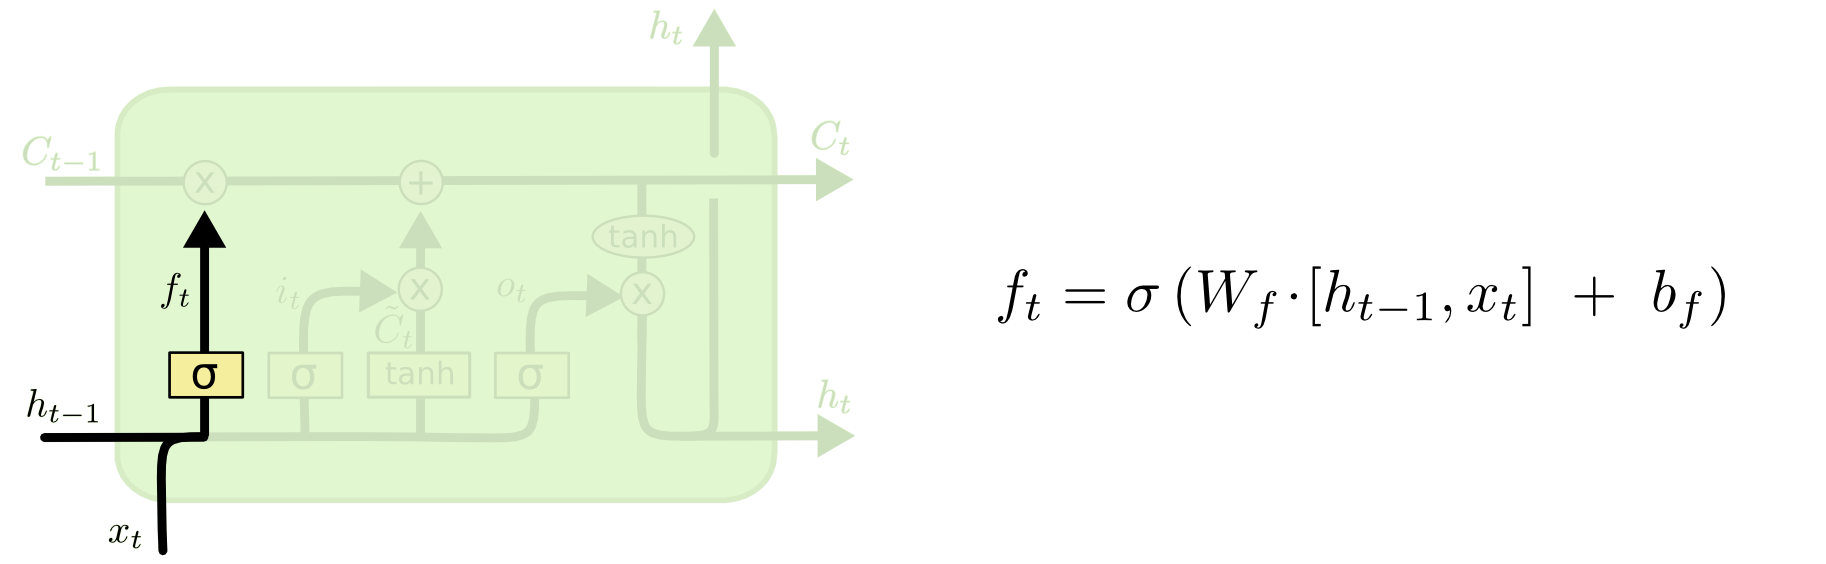
\includegraphics[scale=0.4]{./img/lstm_fog}
			\end{center}
		 \item Input Gate
			\begin{center}
				 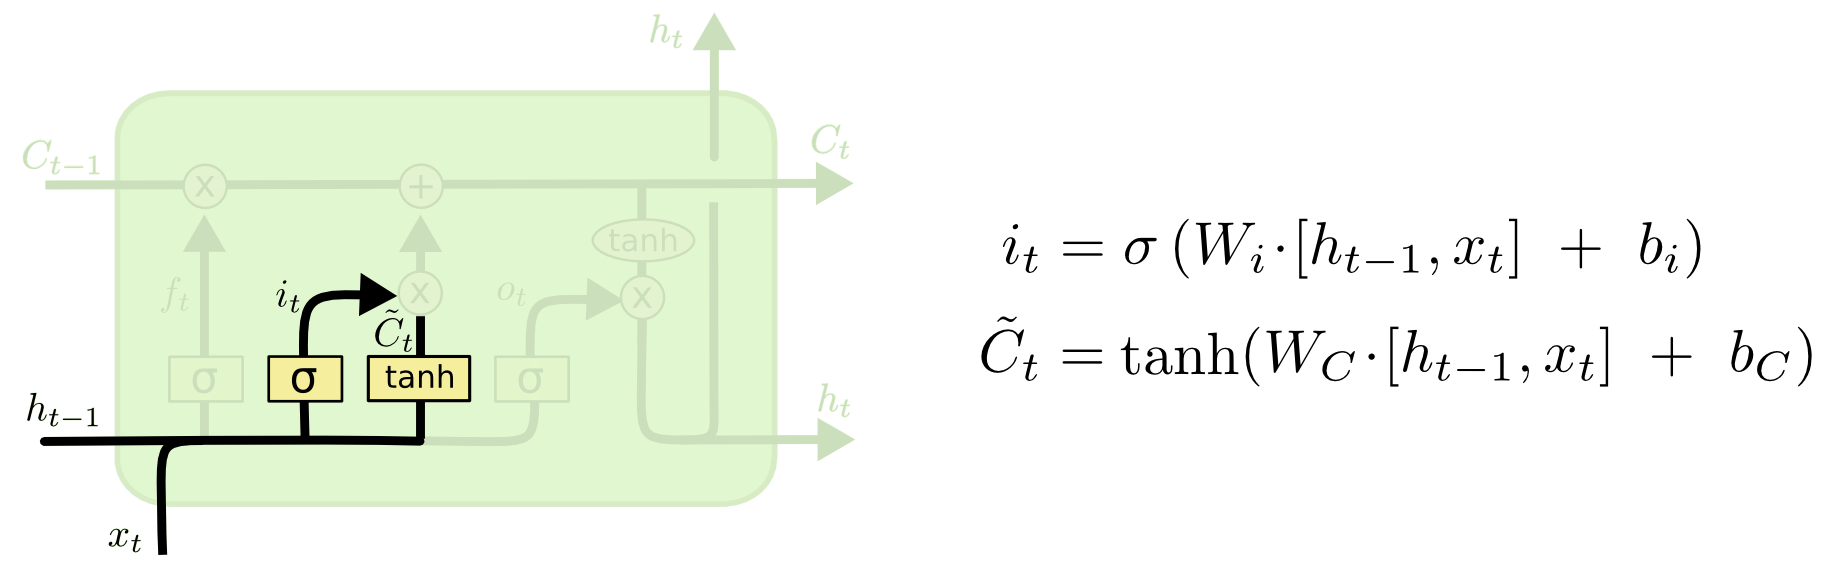
\includegraphics[scale=0.4]{./img/lstm_in}
			\end{center}
	\end{itemize}
\end{frame}

\begin{frame}{Dealing with long term dependences means LSTM}
		\begin{itemize}
			 \item Cell update 
			\begin{center}
				 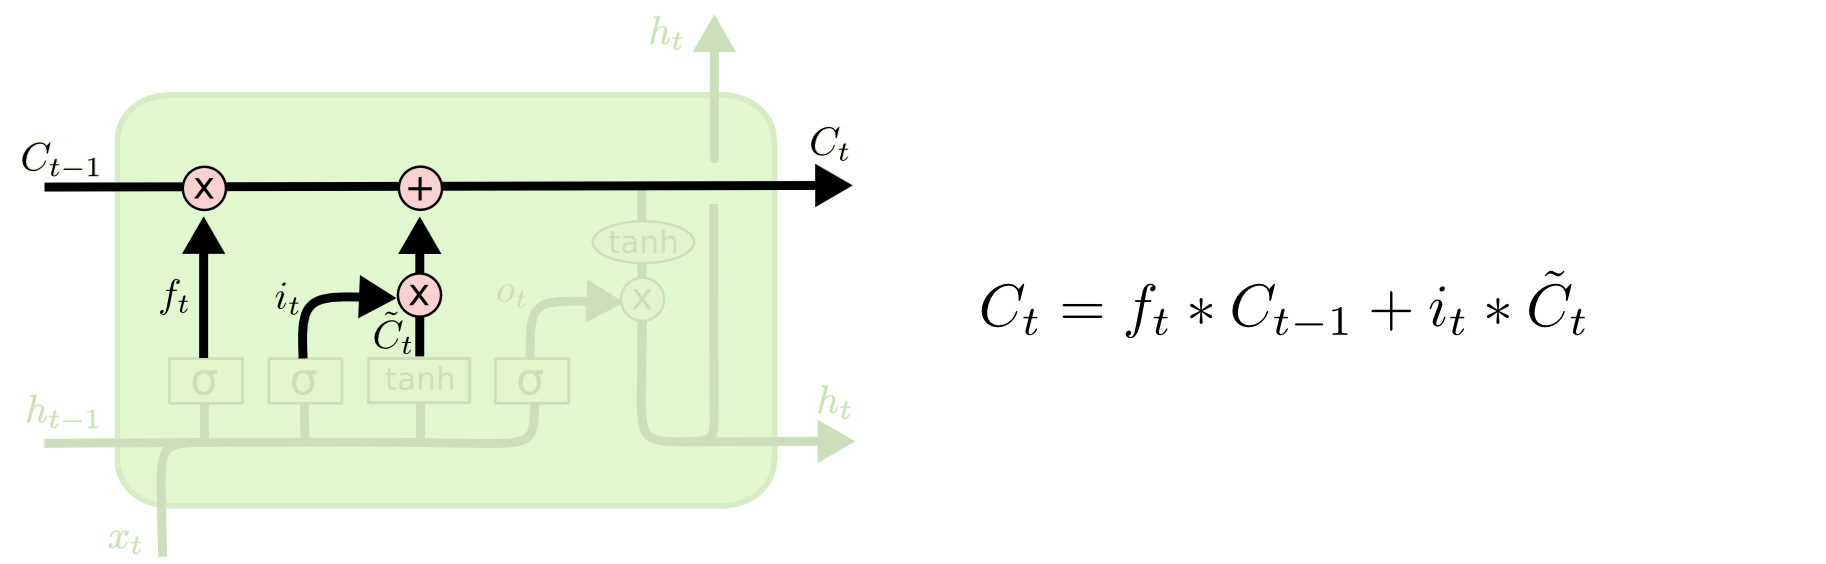
\includegraphics[scale=0.4]{./img/lstm_cell}
			\end{center}
			 \item Output Gate
			\begin{center}
				 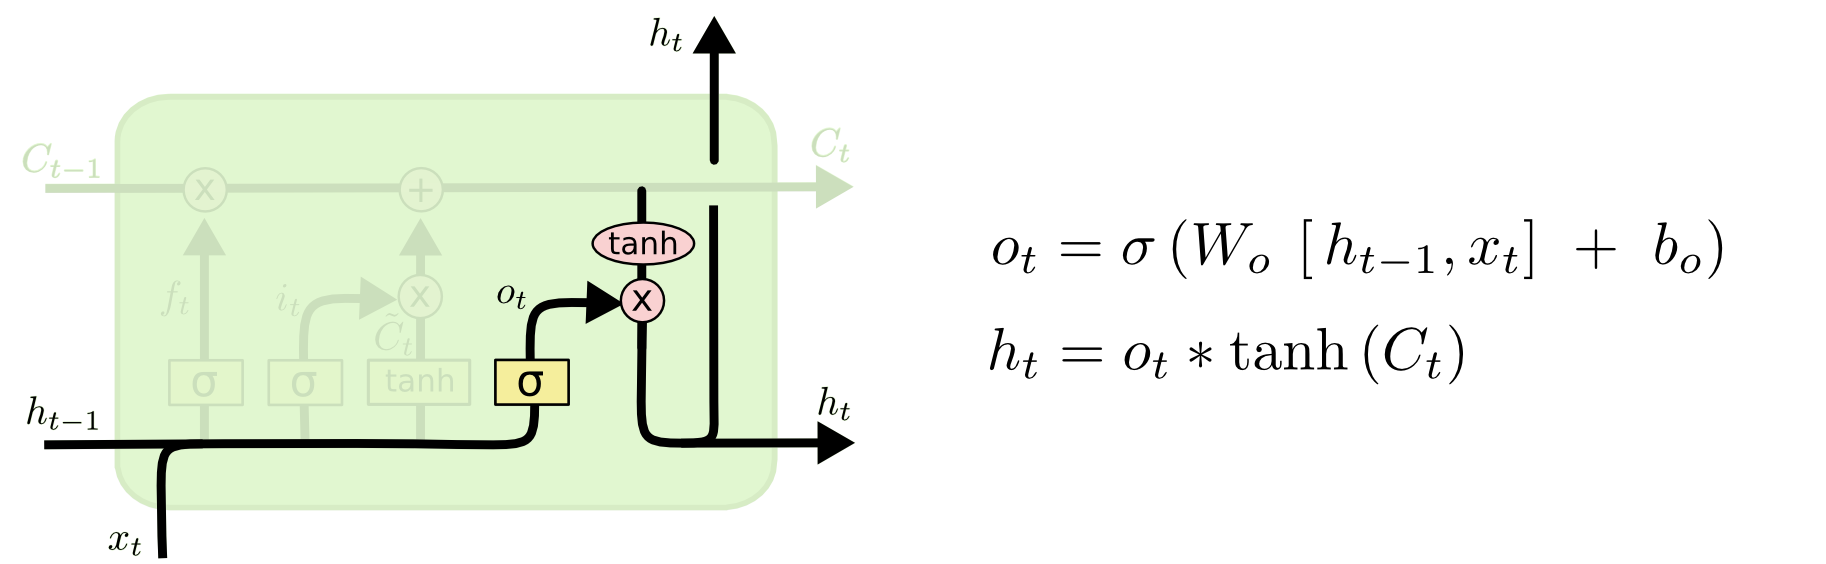
\includegraphics[scale=0.4]{./img/lstm_out}
			\end{center}
		\end{itemize}
\end{frame}

\begin{frame}{Dealing with long term dependences means LSTM}
	\begin{center}
		 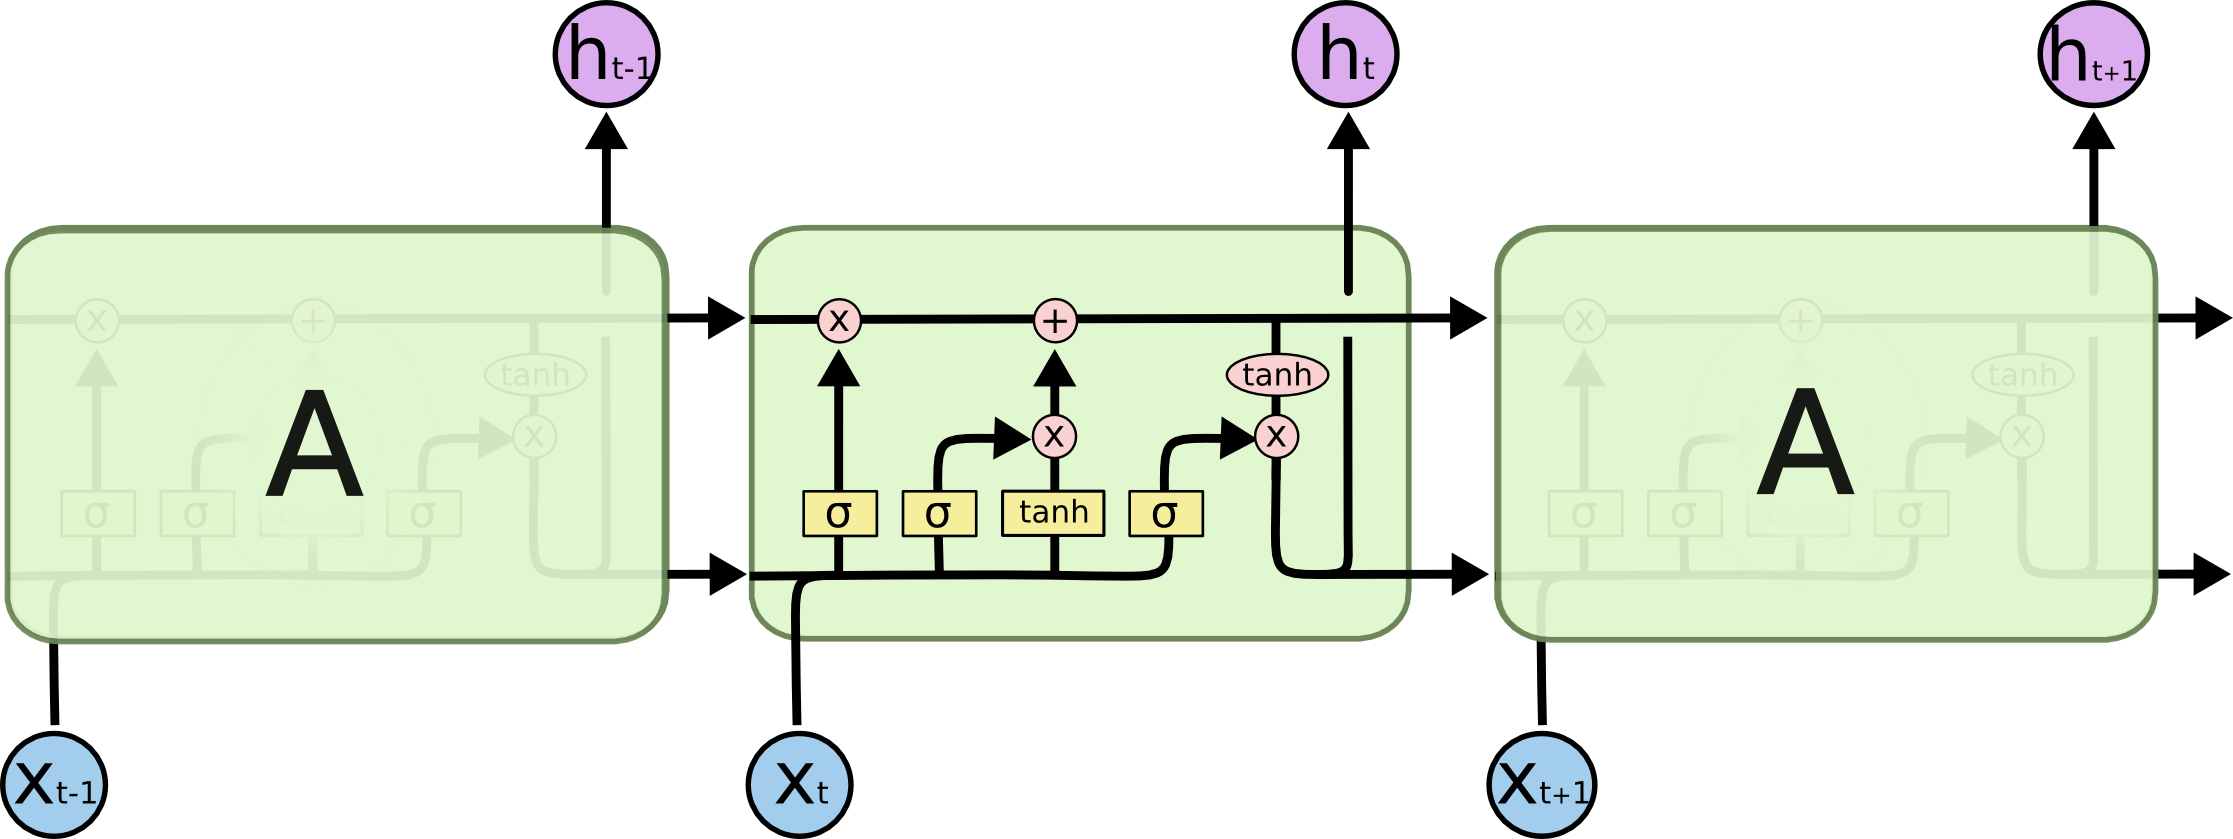
\includegraphics[scale=0.4]{./img/lstm_full}
	\end{center}
\end{frame}

\begin{frame}{Gradient Vanishing in LSTM}
	\begin{center}
		 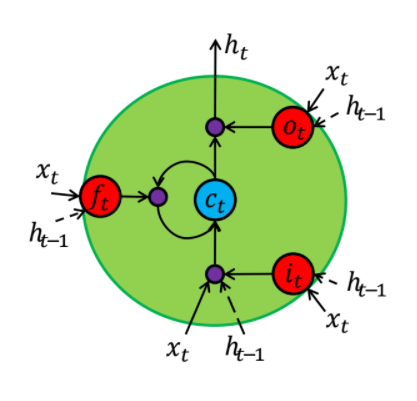
\includegraphics[scale=0.4]{./img/lstm}
	\end{center}
 	$$c_t = f_t\cdot c_{t-1} + t_t\cdot g(W_xx_t+W_ch_{t-1}+b_c),~~~~~h_t = o_t\cdot(c_t)$$
 	$$\frac{\partial c_{t+1} }{\partial c_t} = f_{k+1}$$
\end{frame}


\begin{frame}{Embedding Layer}
	\begin{itemize}
		 \item What the main difference between words and pictures?
		 \item Number of all words in much less then in picture 
		 \item So we can map identity vector for each word
		 \begin{center}
			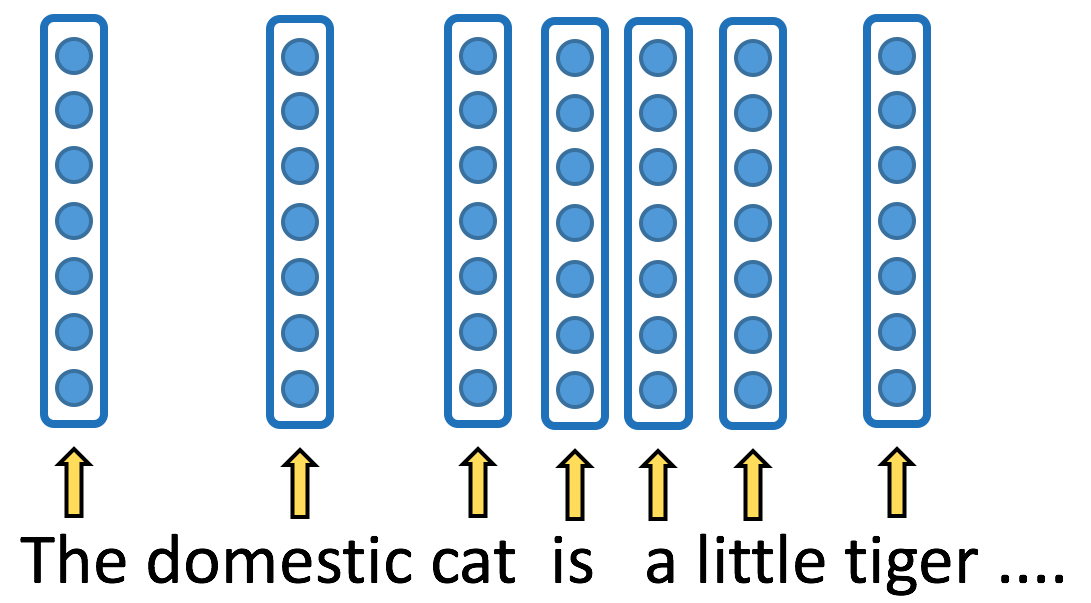
\includegraphics[scale=0.2]{./img/text_repr}
		\end{center}
		 \item Let's initial with random noise
		 \item So, we can evaluate gradient by word vectors
		 \item  word vectors are just a model parameters 
	\end{itemize}
\end{frame}



\begin{frame}[fragile]{Practical Cases}
	\begin{itemize}
		 \item Different tasks type 
		 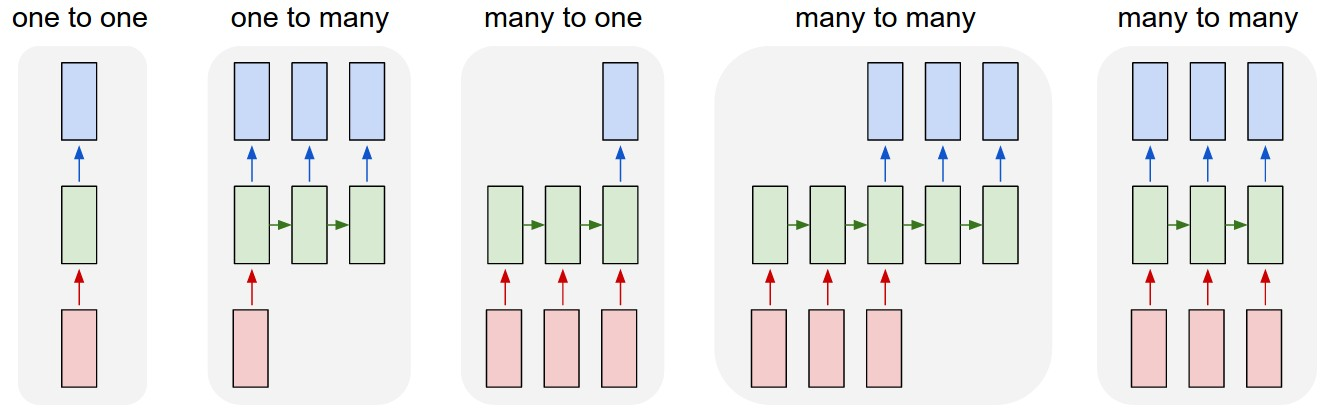
\includegraphics[scale=0.3]{./img/diags}
		 \item Ho to code it
		 
\begin{minted}[fontsize=\small, frame=lines,
framesep=2mm]{python}
decoder = lasagne.layers.LSTMLayer(
    np.opes(batch, seq, vectors), num_units=100, 
    cell_init=smth, grad_clipping=5)
\end{minted}
		
	\end{itemize}
\end{frame}

\begin{frame}{Text/Handwritten Generation}
		\begin{center}
			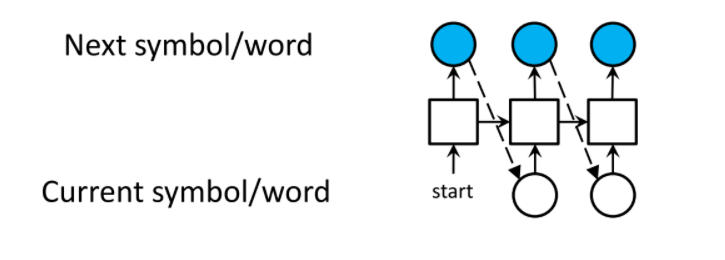
\includegraphics[scale=0.4]{./img/textgen}
		\end{center}
	
	\begin{itemize}
	\item \href{http://karpathy.github.io/2015/05/21/rnn-effectiveness/}{http://karpathy.github.io/2015/05/21/rnn-effectiveness/}
		
	\item \href{http://www.cs.toronto.edu/~graves/handwriting.html}{http://www.cs.toronto.edu/~graves/handwriting.html}
		
	\end{itemize}
\end{frame}

\begin{frame}{Sequence generation}
	\begin{center}
		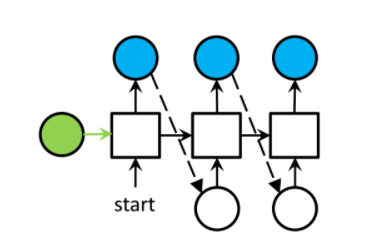
\includegraphics[scale=0.4]{./img/ic}
	\end{center}
	
	\begin{itemize}
		\item\href{http://www.cs.toronto.edu/~nitish/nips2014demo/index.html}{http://www.cs.toronto.edu/~nitish/nips2014demo/index.html}
		
		\item \href{http://cs.stanford.edu/people/karpathy/deepimagesent/generationdemo/}{cs.stanford.edu/people/karpathy/deepimagesent/generationdemo/}
		
	\end{itemize}
\end{frame}

\begin{frame}{Sequence classification}
	\begin{center}
		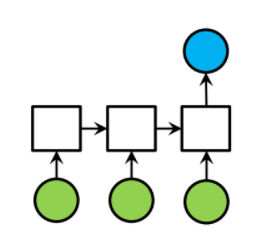
\includegraphics[scale=0.3]{./img/sc}
		
		
		 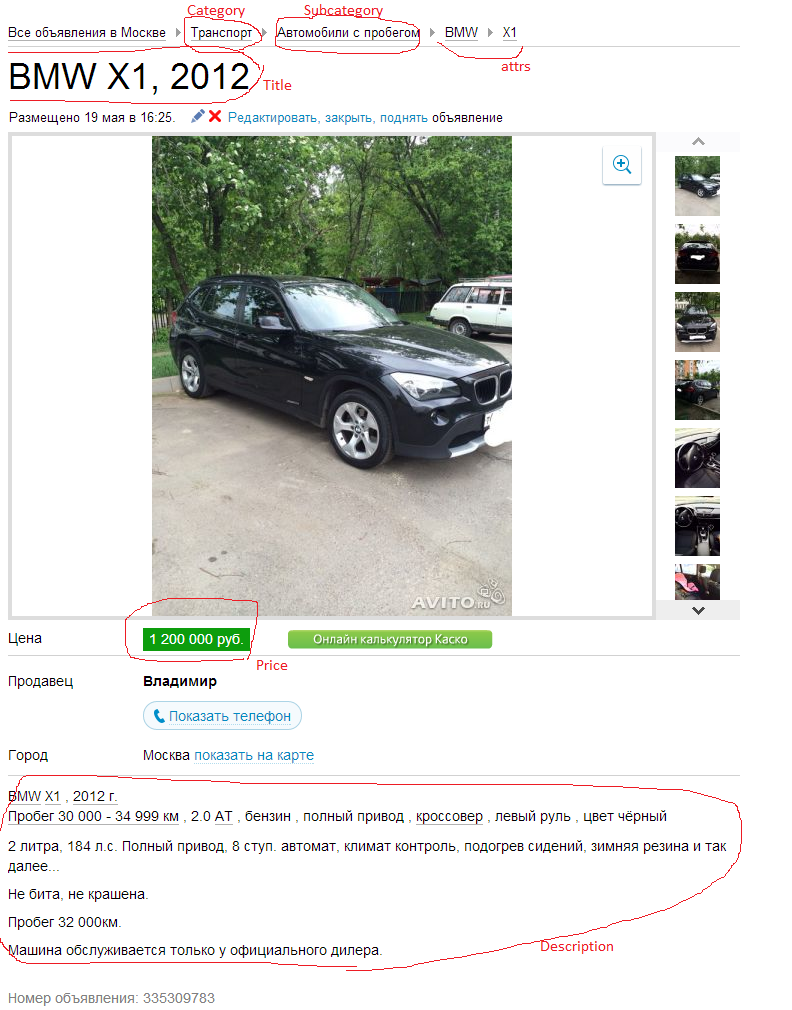
\includegraphics[scale=0.2]{./img/avito} ~~  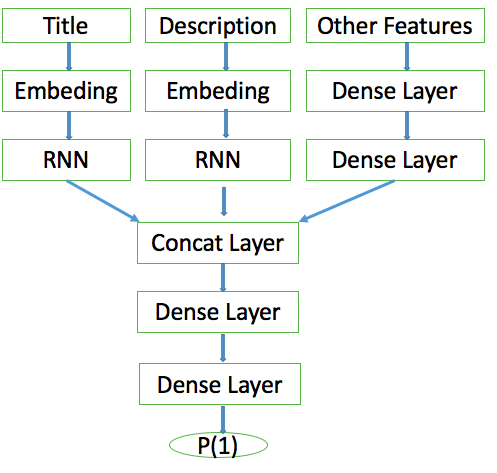
\includegraphics[scale=0.3]{./img/clf}
	\end{center}
\end{frame}

\begin{frame}{Sequence2Sequence Machine Translation }
		\begin{itemize}
			\item   Coding input sentence and generate output
				 \begin{center}
					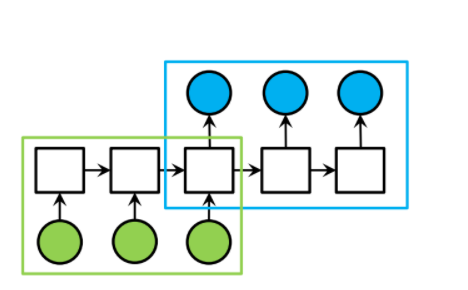
\includegraphics[scale=0.2]{./img/transl.png}
				\end{center}
			\item   Add attention mechanize
				 \begin{center}
					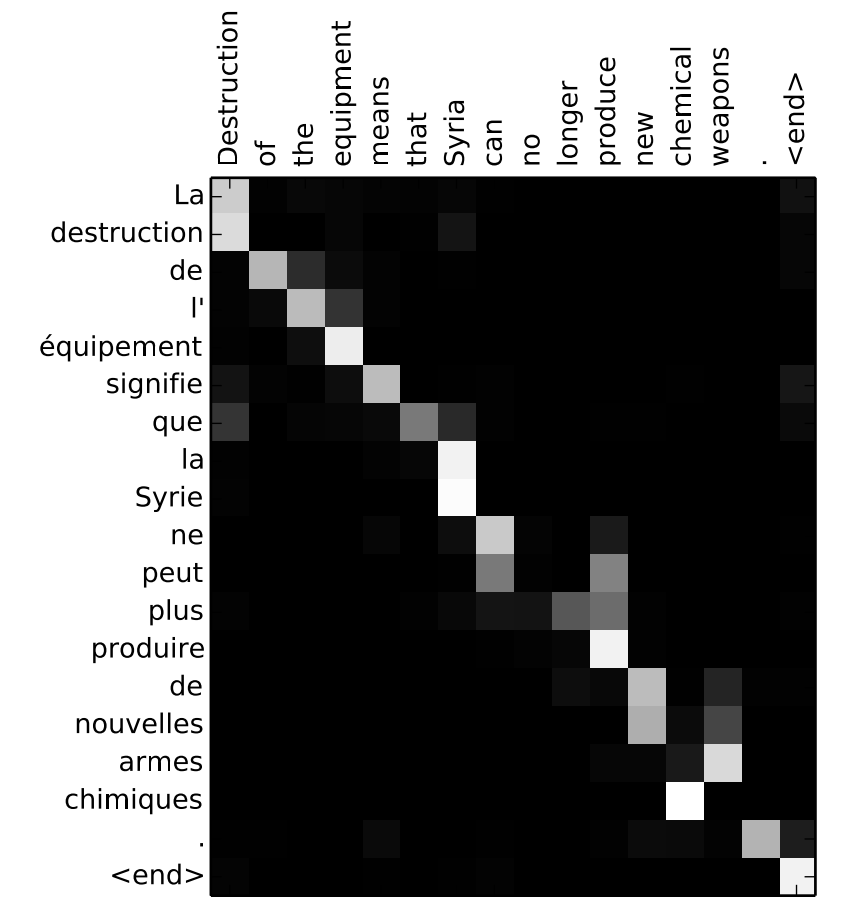
\includegraphics[scale=0.32]{./img/tr.png}
				\end{center}
		\end{itemize}


\end{frame}

\begin{frame}{Recap}
	\begin{itemize}
		\item Recurrent Deep Neural nets are great
		\item RNN has achieved many state of the art awards
		\item Input and output may have any length 
		\item It can be combine with convolution DNN
		\item It's Easy to code it by yourself with any DL framework
		\item Link's
			\begin{itemize}
				\item \href{http://colah.github.io/posts/2015-08-Understanding-LSTMs/}{http://colah.github.io/posts/2015-08-Understanding-LSTMs/}
				\item \href{http://www.machinelearning.ru/wiki/index.php?title=Dl} {http://www.machinelearning.ru/wiki/index.php?title=Dl} 
				\item \href{www.deeplearningbook.org}{www.deeplearningbook.org}
			\end{itemize}
	\end{itemize}
\end{frame}


\end{document}

